\mode*

\section{What's an interface?}

\begin{frame}
  \begin{definition}[Interface, n.\footnote{Oxford English Dictionary, 1989}]
    \begin{enumerate}
      \item A surface lying between two portions of matter or space, and 
        forming their common boundary.
      \item \emph{transf.} and \emph{fig.}
        \begin{enumerate}
          \item A means or place of interaction between two systems, 
            organizations, etc.; a meeting-point or common ground between two 
            parties, systems, or disciplines; also, interaction, liaison, 
            dialogue.
          \item (An) apparatus designed to connect two scientific instruments, 
            devices, etc., so that they can be operated jointly.
        \end{enumerate}
    \end{enumerate}
  \end{definition}
\end{frame}

\begin{frame}
  \begin{block}{Construction}
    \begin{itemize}
      \item inter-: from Latin, meaning between.
      \item face: from Latin \emph{facies}; meaning appearance, form or figure.
    \end{itemize}
  \end{block}
\end{frame}

\section{Interfaces in CS}

\subsection{Graphical User Interfaces (GUIs)}

\begin{frame}
  \begin{exercise}
    \begin{itemize}
      \item Based on the construction of the term, what does Graphical User 
        Interface mean?
    \end{itemize}
  \end{exercise}
\end{frame}

\begin{frame}
  \begin{figure}
    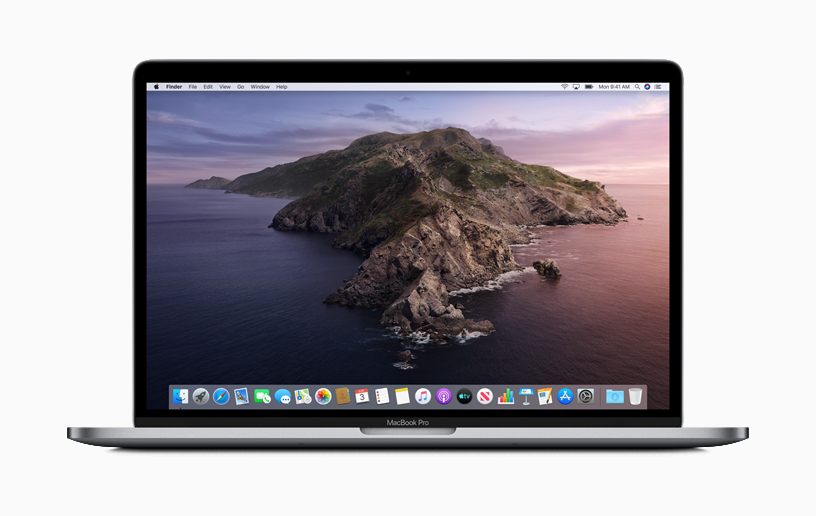
\includegraphics[height=0.8\textheight]{fig/macos.jpg}
    \caption{The macOS Catalina user interface.}
  \end{figure}
\end{frame}

\begin{frame}
  \begin{figure}
    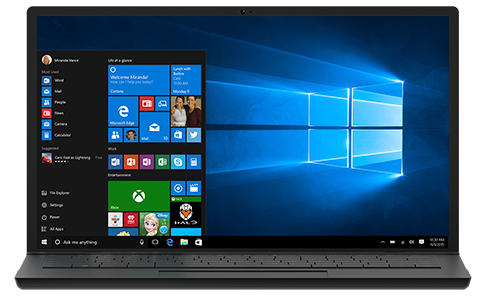
\includegraphics[height=0.8\textheight]{fig/windows10-laptop.png}
    \caption{The Windows 10 user interface.}
  \end{figure}
\end{frame}

\begin{frame}
  \begin{figure}
    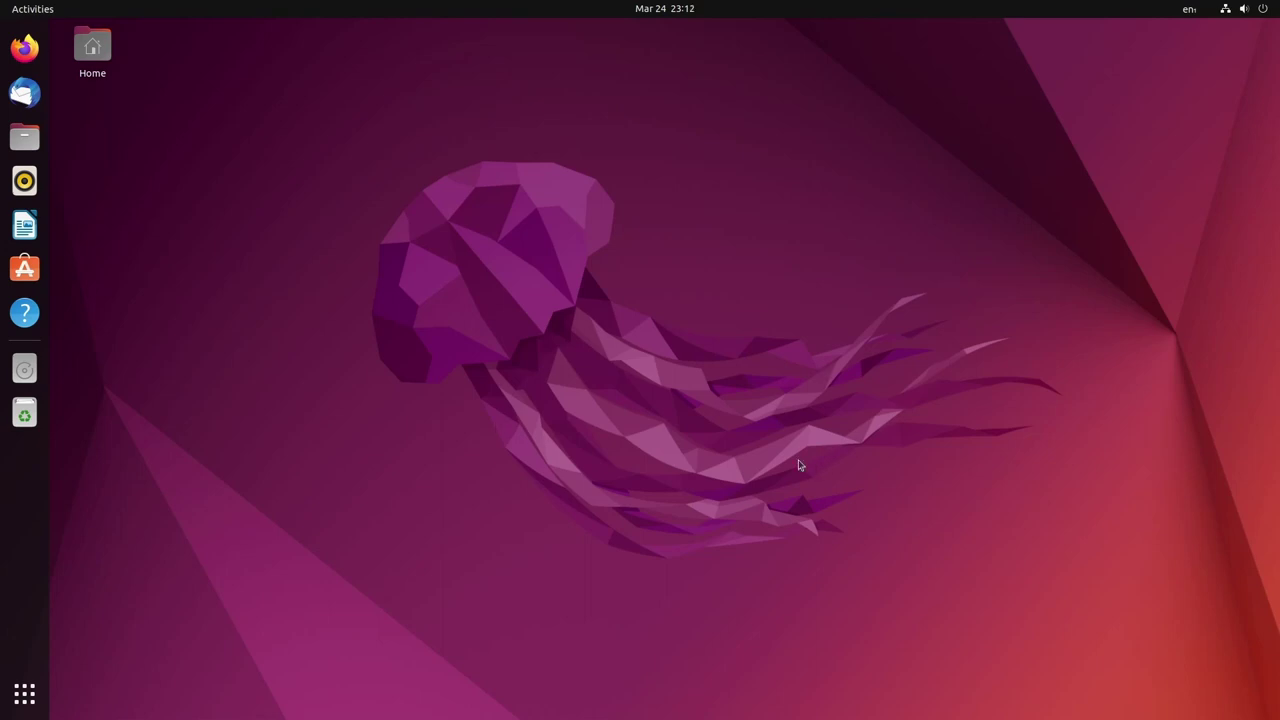
\includegraphics[width=\columnwidth]{fig/ubuntu.png}
    \caption{The Ubuntu 22.04 user interface.}
  \end{figure}
\end{frame}

%\begin{frame}
%  \begin{figure}
%    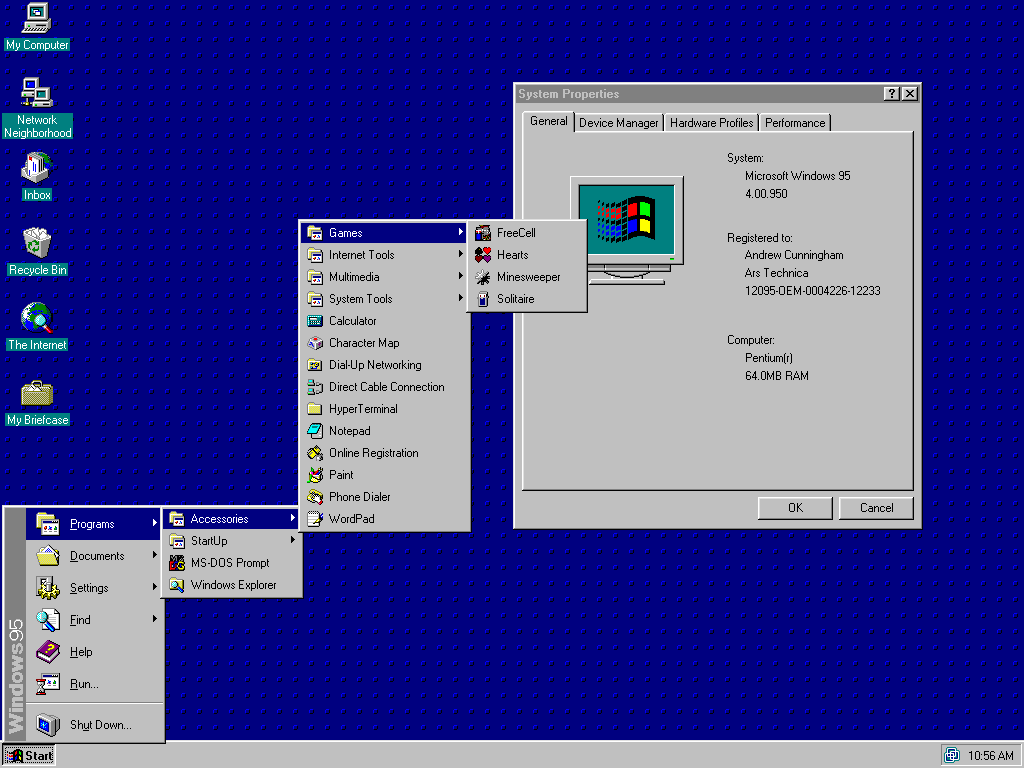
\includegraphics[height=0.8\textheight]{fig/windows95.png}
%    \caption{The Windows 95 user interface.}
%  \end{figure}
%\end{frame}

\begin{frame}
  \begin{figure}
    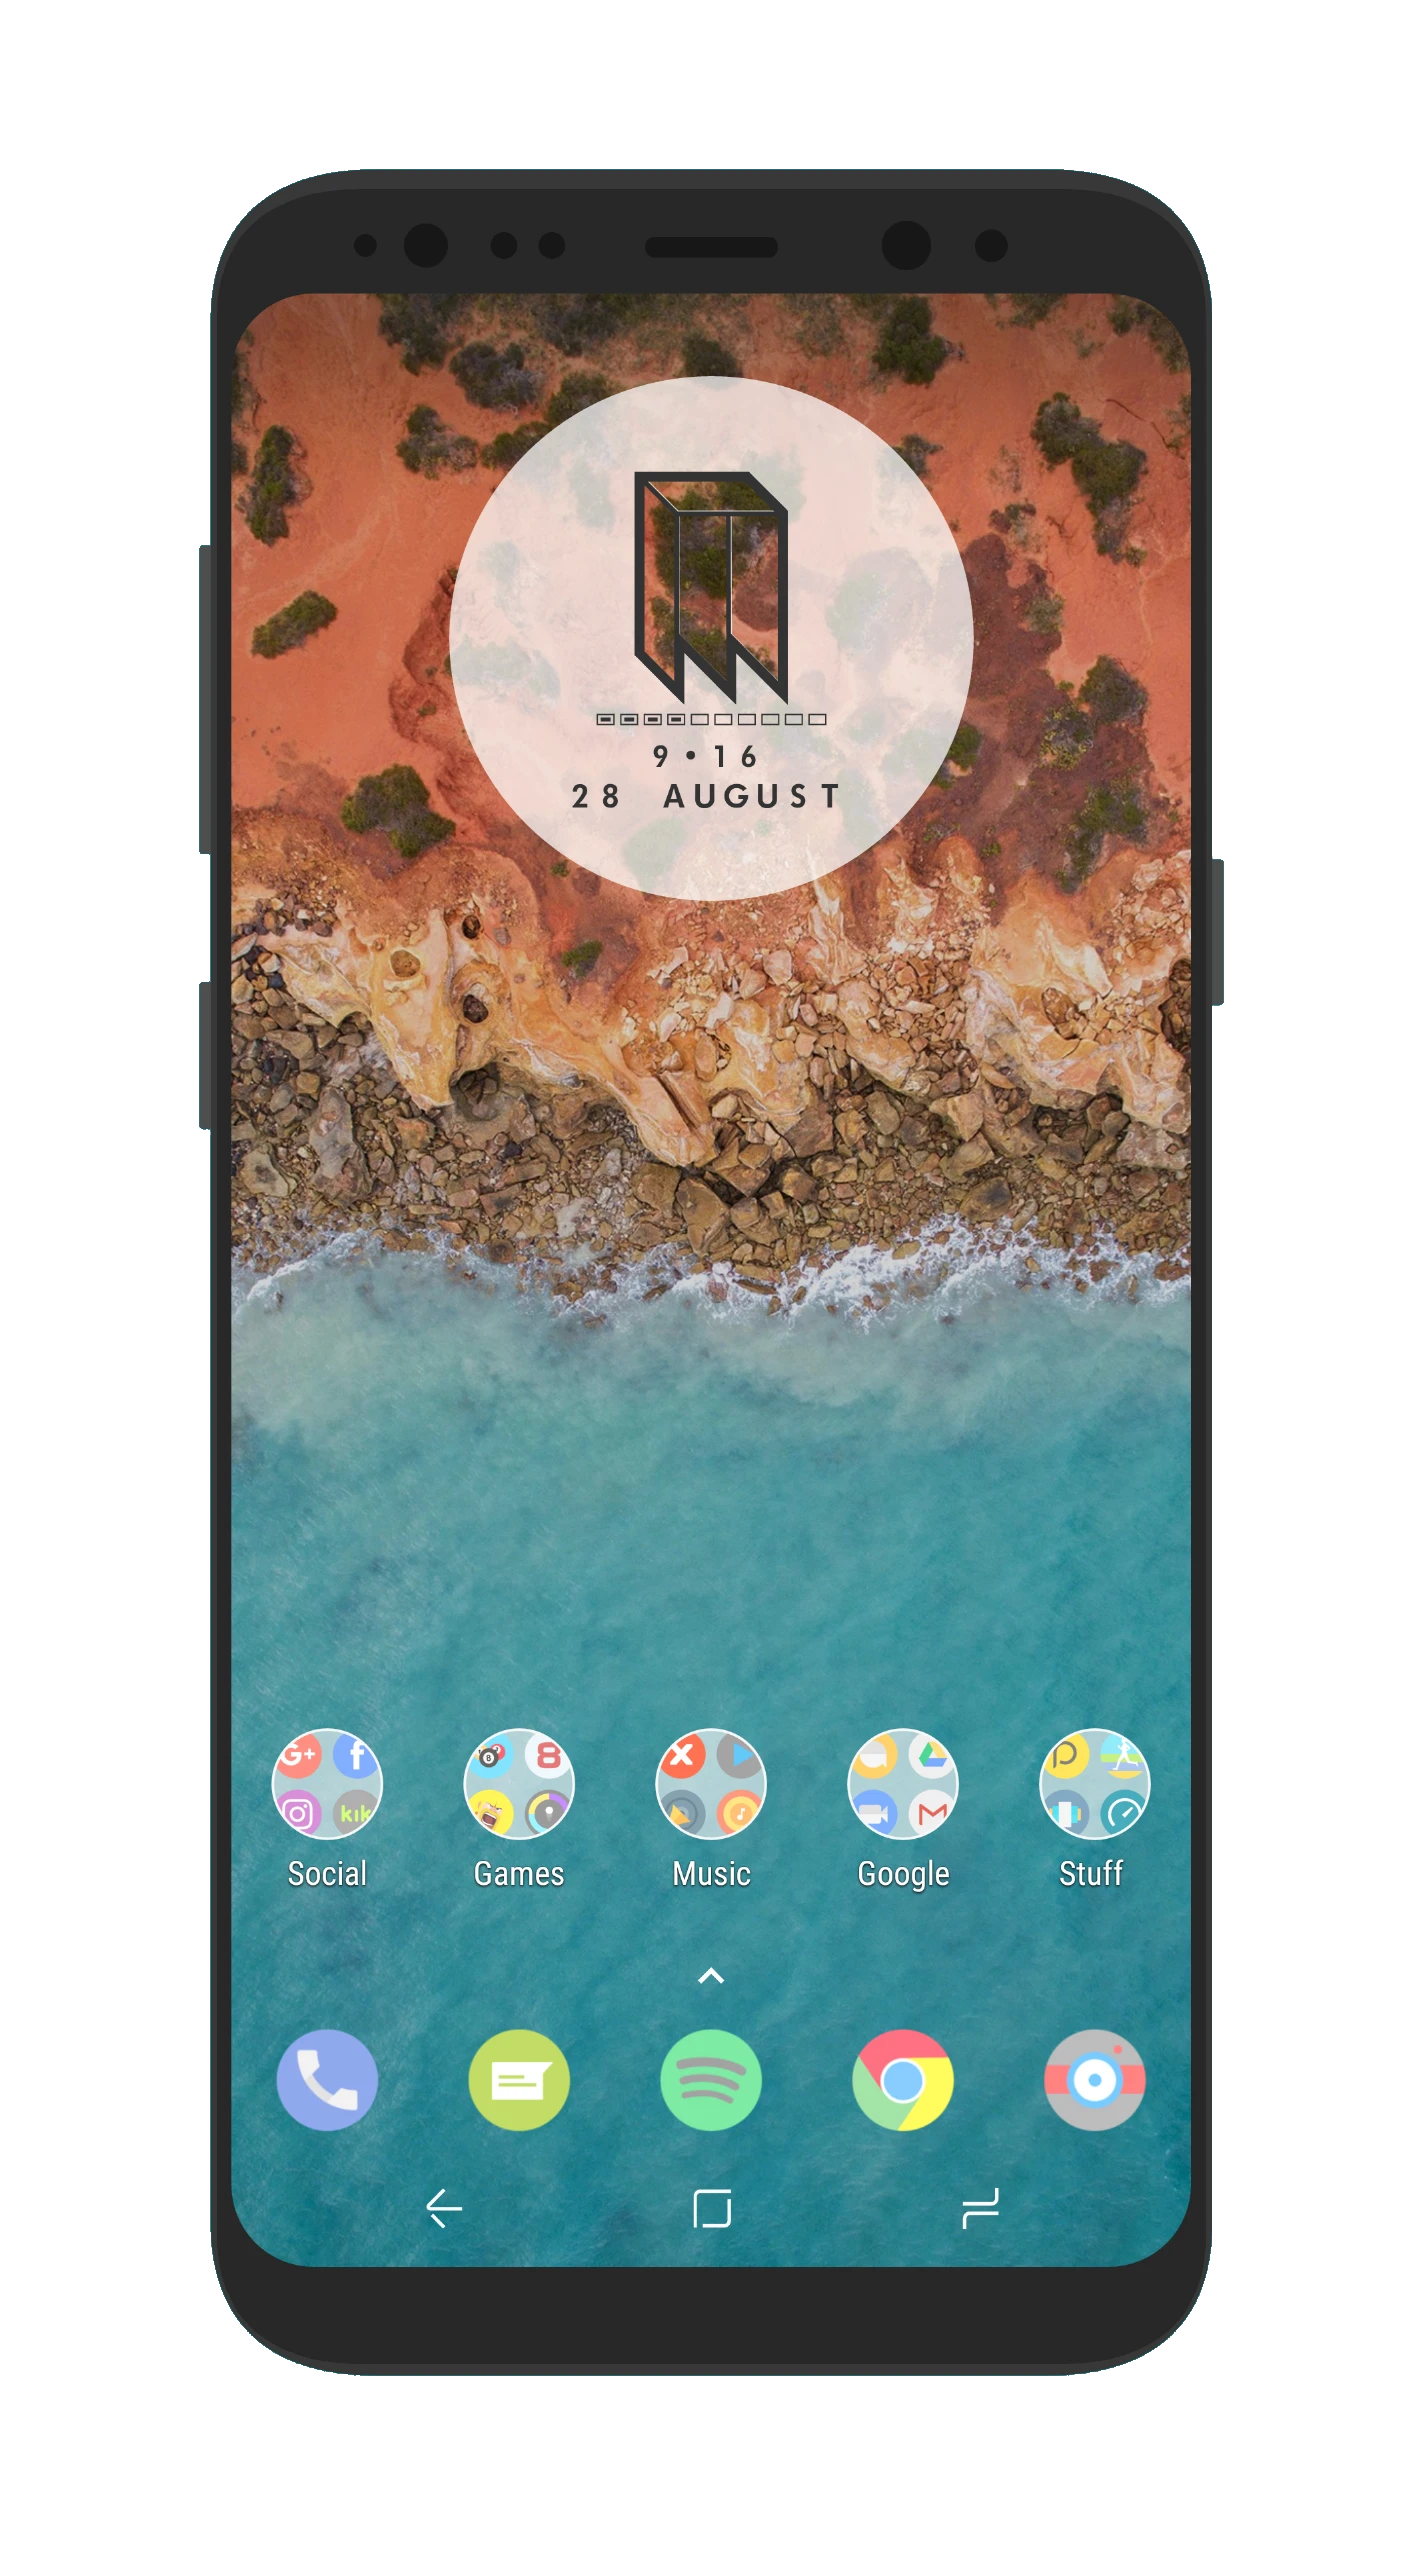
\includegraphics[height=0.8\textheight]{fig/android.png}
    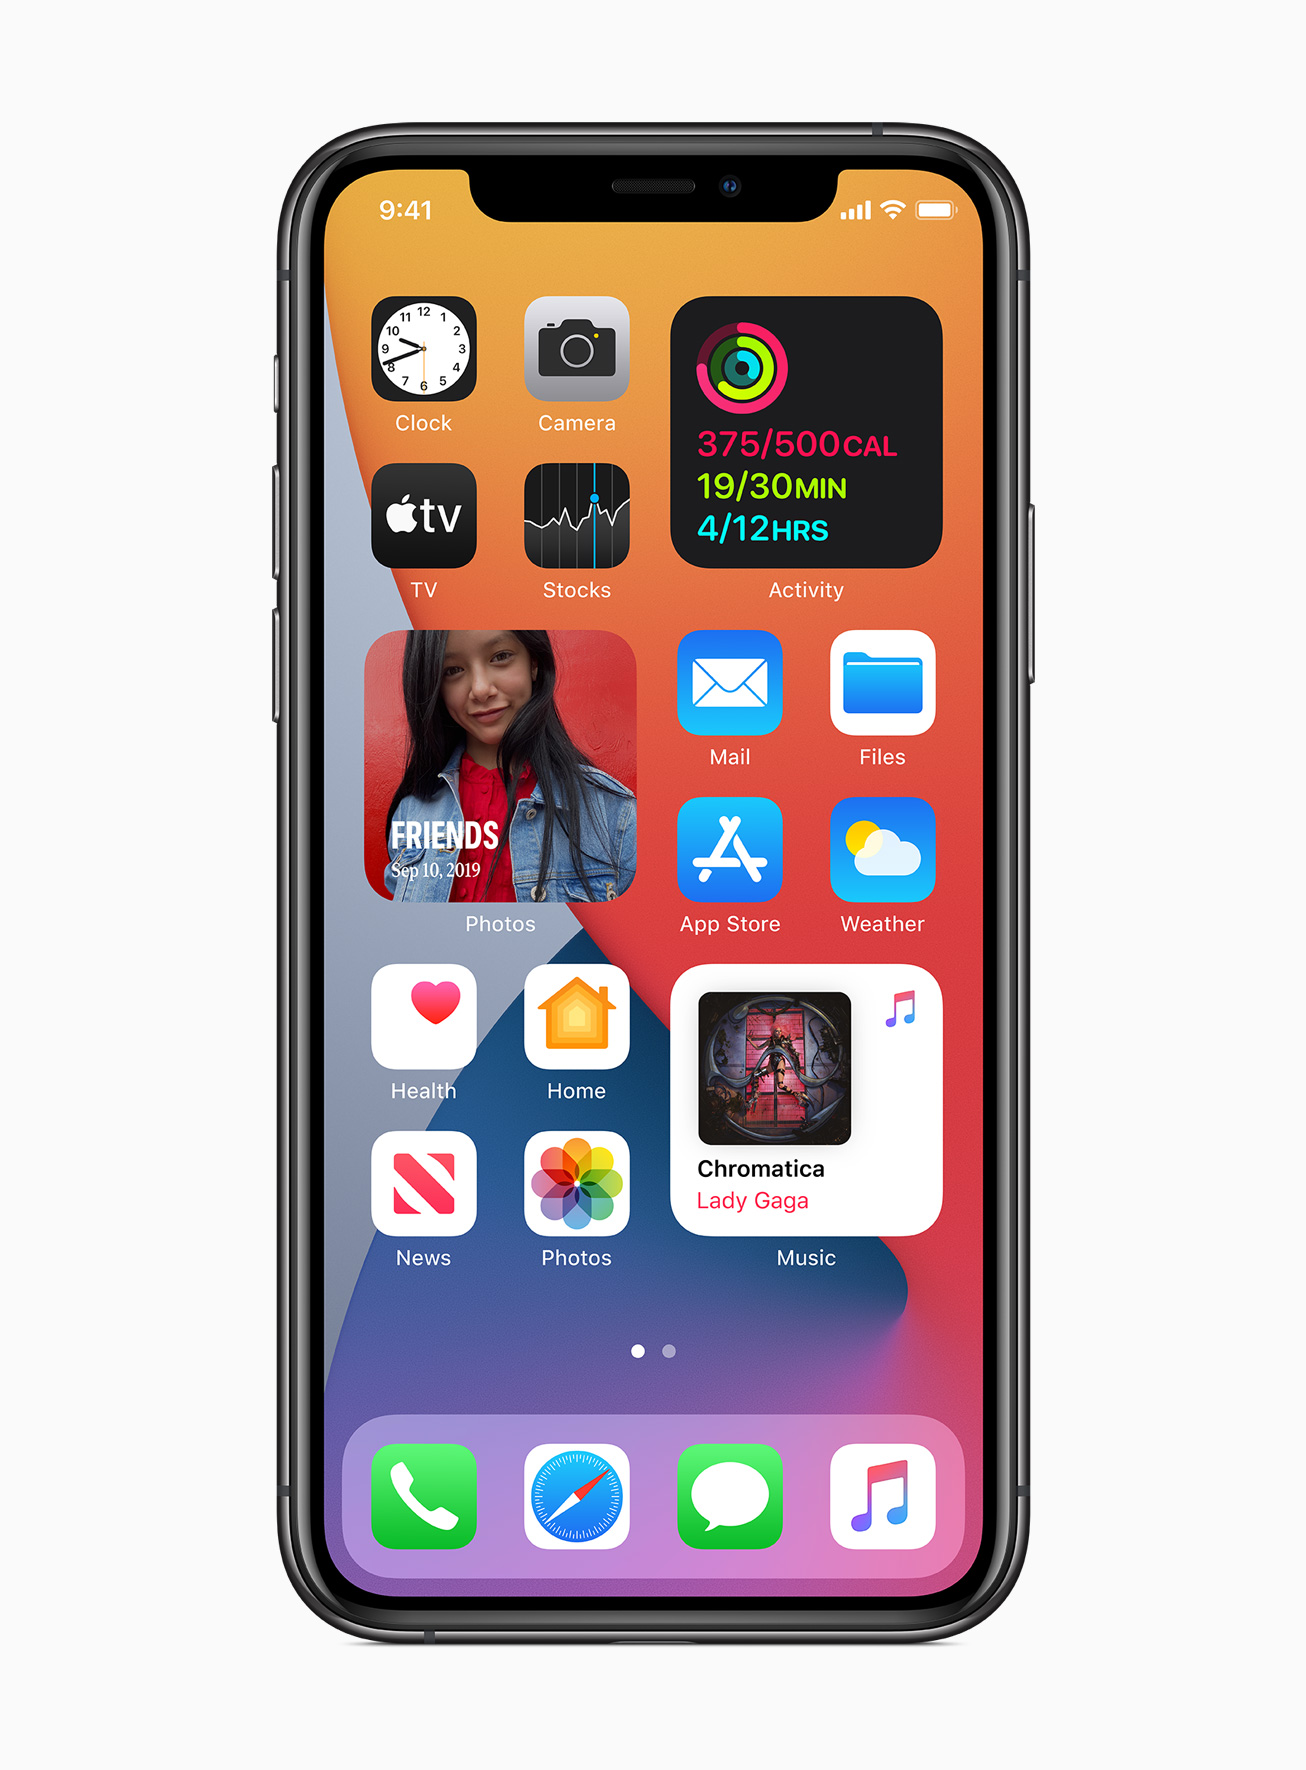
\includegraphics[height=0.8\textheight]{fig/ios14.jpg}
    \caption{Android and iOS touch-based interfaces.}
  \end{figure}
\end{frame}

%\begin{frame}
%  \begin{figure}
%    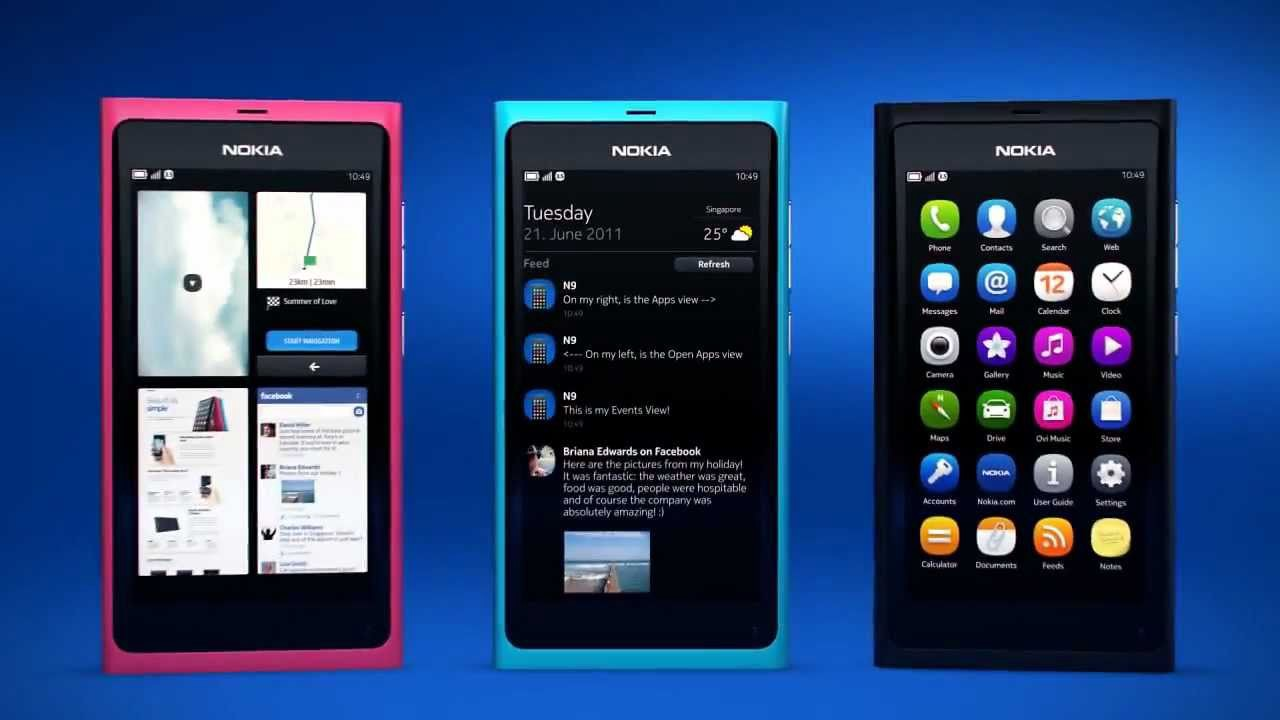
\includegraphics[width=\columnwidth]{fig/nokia-n9.jpg}
%    \caption{Gesture-based, touch interface of Nokia N9.}
%  \end{figure}
%\end{frame}

\subsection{Command-Line Interfaces (CLIs)}

\begin{frame}
  \begin{exercise}
    \begin{itemize}
      \item Based on the construction of the term, what does Command-Line 
        Interface mean?
    \end{itemize}
  \end{exercise}
\end{frame}

\begin{frame}
  \begin{figure}
    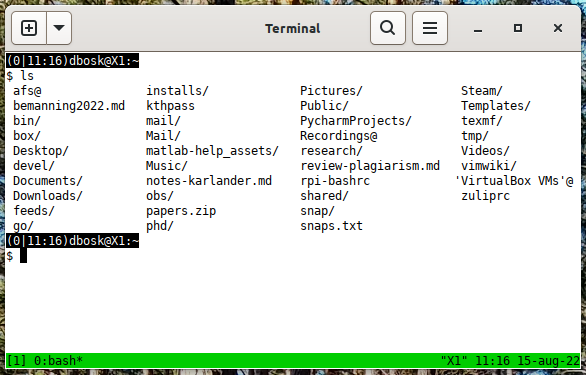
\includegraphics[height=0.8\textheight]{fig/files-ls.png}
    \caption{Listing files in CLI on Ubuntu (same on macOS).}
  \end{figure}
\end{frame}

\begin{frame}
  \begin{figure}
    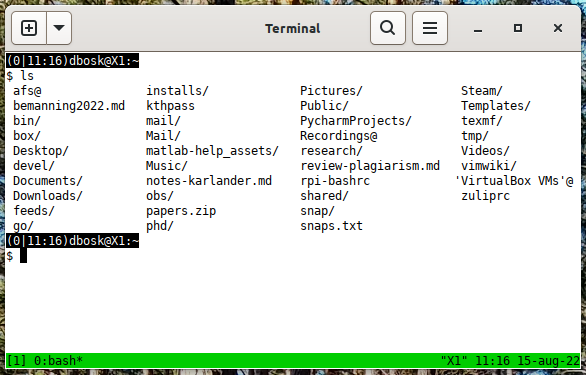
\includegraphics[width=0.4\columnwidth]{fig/files-ls.png}
    \hfill
    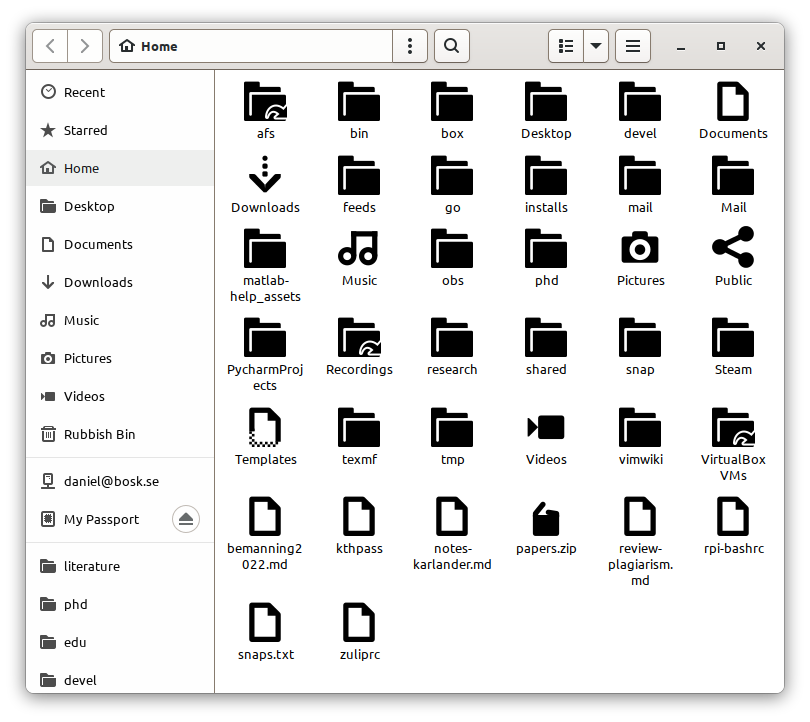
\includegraphics[width=0.5\columnwidth]{fig/files.png}
    \caption{Listing files in CLI (left) and GUI (right) on Ubuntu.}
  \end{figure}
\end{frame}

\begin{frame}
  \begin{figure}
    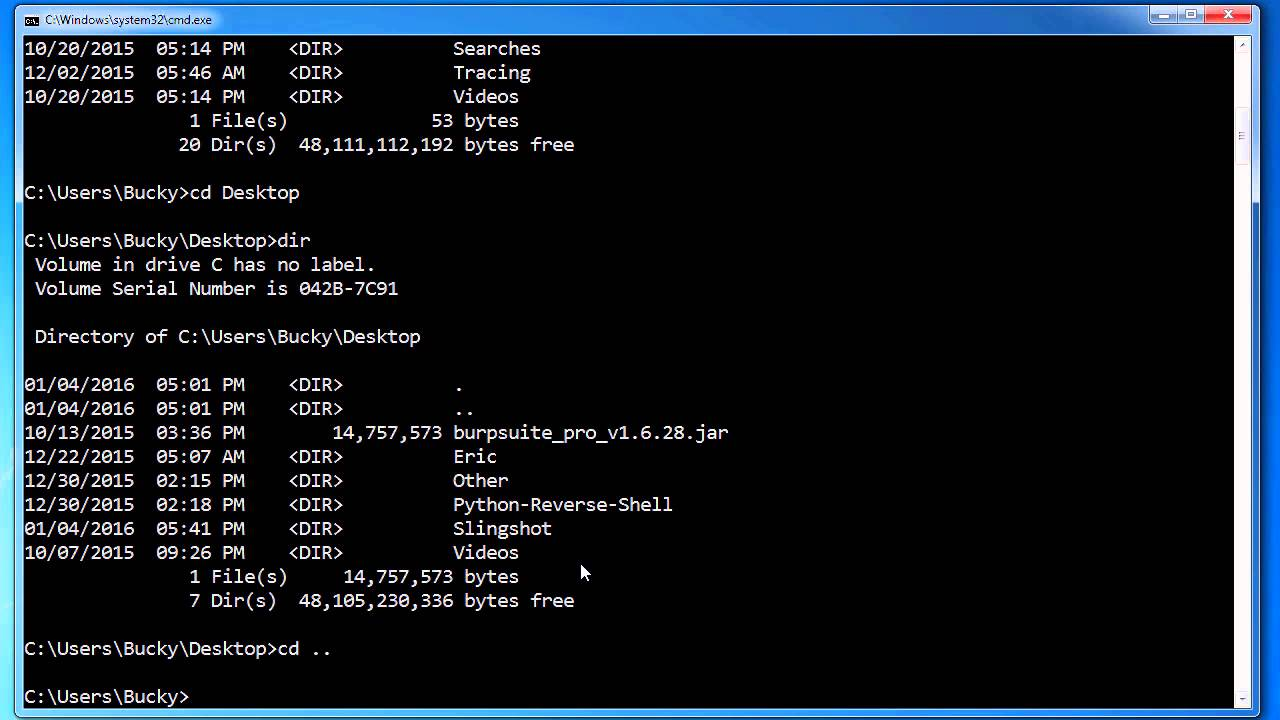
\includegraphics[height=0.8\textheight]{fig/dir.jpg}
    \caption{Listing files in CLI on Windows (command interpreter).}
  \end{figure}
\end{frame}

\begin{frame}
  \begin{figure}
    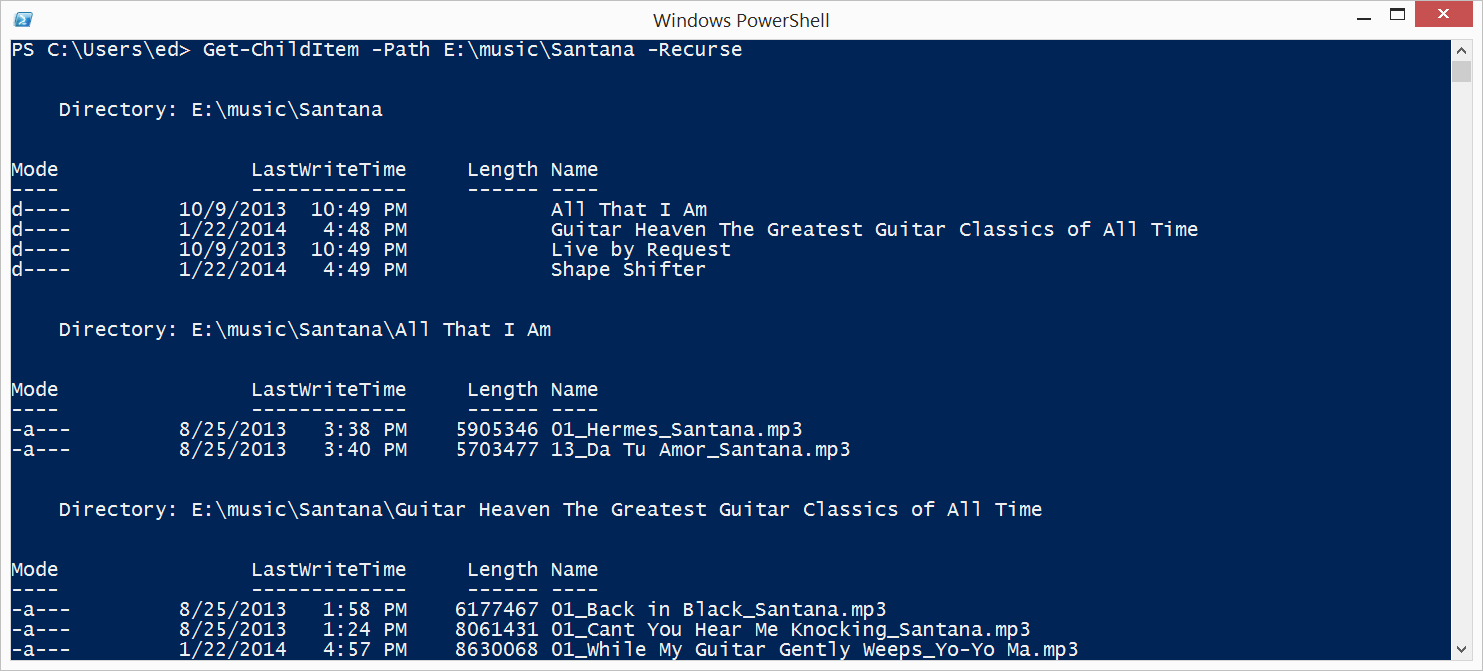
\includegraphics[width=\columnwidth]{fig/GetChildItem.png}
    \caption{Listing files in CLI on Windows (PowerShell).}
  \end{figure}
\end{frame}

\begin{frame}
  \begin{exercise}
    \begin{enumerate}
      \item List some differences between Graphical User Interfaces and 
        Command-Line Interfaces.
      \item What would you say is the crucial difference?
    \end{enumerate}
  \end{exercise}
\end{frame}

\subsection{Application-Programming Interfaces (APIs)}

\begin{frame}
  \begin{exercise}
    \begin{itemize}
      \item Based on the construction of the term, what does 
        Application-Programming Interface mean?
    \end{itemize}
  \end{exercise}
\end{frame}

\begin{frame}
  \begin{columns}
    \begin{column}{0.5\columnwidth}
      \begin{block}{\texttt{ls-api.py}}
        \inputminted[fontsize=\tiny,linenos,highlightlines={1,4}]{python}{code/ls-api.py}
      \end{block}
    \end{column}
    \begin{column}{0.5\columnwidth}
      \begin{figure}
        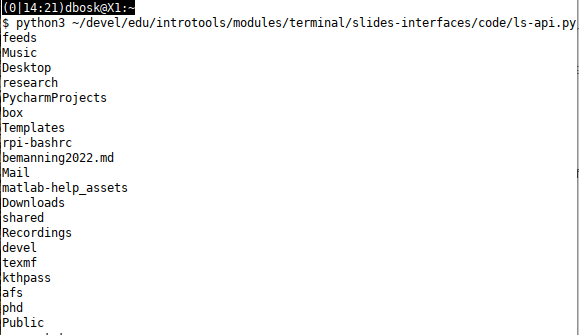
\includegraphics[width=\columnwidth]{fig/ls-api-out.png}
        \caption{Output of \texttt{ls-api.py}.}
      \end{figure}
    \end{column}
  \end{columns}
\end{frame}

\begin{frame}
  \begin{columns}
    \begin{column}{0.7\columnwidth}
      \begin{block}{\texttt{ls.py}}
        \inputminted[fontsize=\tiny,linenos,highlightlines={1-2,5,7}]{python}{code/ls.py}
      \end{block}
    \end{column}
    \begin{column}{0.3\columnwidth}
      \begin{figure}
        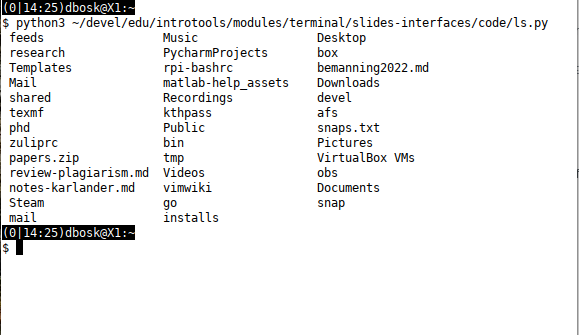
\includegraphics[width=\columnwidth]{fig/ls-out.png}
        \caption{Output of \texttt{ls.py}.}
      \end{figure}
    \end{column}
  \end{columns}
\end{frame}

\begin{frame}
  \begin{exercise}
    \begin{itemize}
      \item Discuss the relations between the different interfaces:
        \begin{itemize}
          \item Graphical User Interface
          \item Command Line Interface
          \item Application Programming Interface
        \end{itemize}
    \end{itemize}
  \end{exercise}
\end{frame}

\begin{frame}[fragile]
  \begin{solution}[Most important]
    \begin{itemize}
      \item GUI is a User Interface (UI).
      \item The API is an interface for writing programs.
      \item CLI is a hybrid; it's a UI, but it can easily be used to write 
        programs.
    \end{itemize}
  \end{solution}

  \begin{example}[Counting the number of files]
    \begin{minted}{bash}
ls | wc -l
    \end{minted}
  \end{example}
\end{frame}

\begin{frame}
  \begin{figure}
    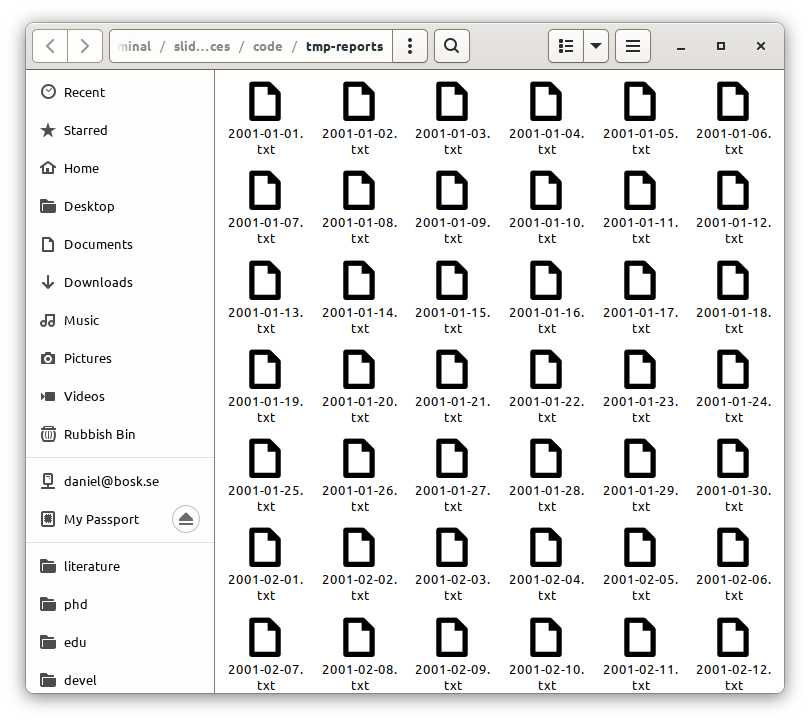
\includegraphics[height=0.5\textheight]{fig/many-reports.png}
    \caption{file explorer showing many dated report files.}
  \end{figure}

  \begin{exercise}[Printing contents of specific files]
    \begin{itemize}
      \item Take the contents of all reports from summers of 2005--2008.
      \item Put into one file.
    \end{itemize}
  \end{exercise}
\end{frame}

\begin{frame}[fragile]
  \begin{figure}
    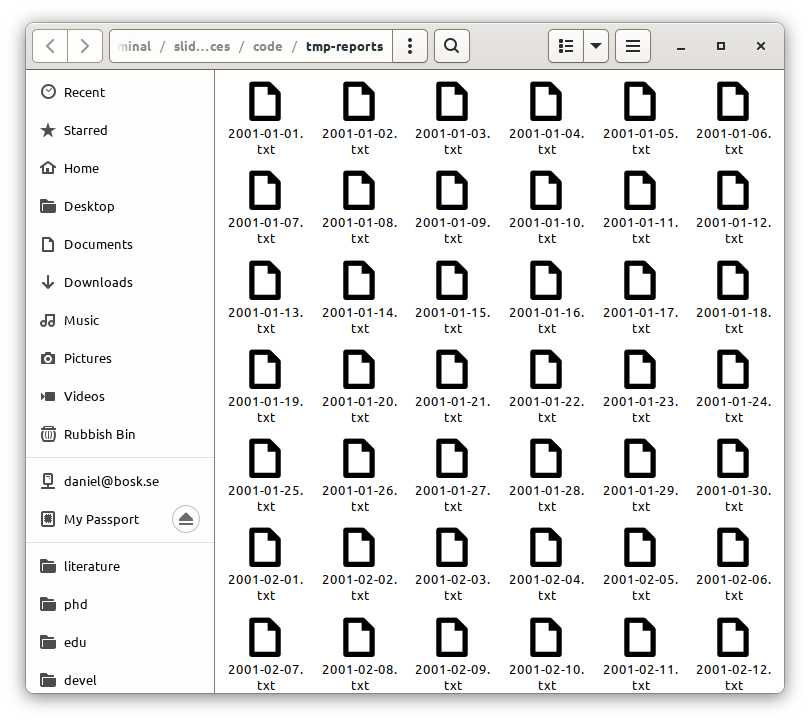
\includegraphics[height=0.5\textheight]{fig/many-reports.png}
    \caption{file explorer showing many dated report files.}
  \end{figure}

  \begin{solution}[CLI-solution: \texttt{summer.sh}]
    \inputminted[firstline=3]{bash}{code/summer.sh}
  \end{solution}
\end{frame}

\begin{frame}
  \begin{remark}[Web services]
    \begin{itemize}
      \item Obviously they have (G)UIs too.
      \item Many web services have APIs too.
    \end{itemize}
  \end{remark}
\end{frame}


\section{More reasons for CLI?}

\begin{frame}
  \begin{example}[Your thesis]
    \begin{itemize}
      \item You might run experiments.
      \item Results are in files.
      \item Sure you could write a program in Python.
    \end{itemize}
  \end{example}
\end{frame}

\begin{frame}
  \begin{example}[Supercomputing]
    \begin{itemize}
      \item Two KTH students had to simulate the Tor network.
      \item Can't be done on a laptop, requires supercomputer (HPC).
      \item Got CPU time on HPC in Linköping.
      \item Only SSH (CLI) access.
    \end{itemize}
  \end{example}

  \pause

  \begin{example}
    \begin{itemize}
      \item Training ML model.
      \item Analyse protein sequences.
      \item \dots
    \end{itemize}
  \end{example}
\end{frame}

\begin{frame}
  \begin{remark}
    \begin{itemize}
      \item All HPCs run using CLIs\footnote{%
          In June 2022, all HPC clusters in the Top 500 ran Linux.
          See top500.org for details.
        }.
      \item All GNU/Linux systems are UNIX-like.
      \item BSD systems are UNIX descendants.
      \item macOS is even a UNIX descendant.
      \item Android is built on Linux.
    \end{itemize}
  \end{remark}

  \pause

  \begin{block}{Operating systems family tree}
    \begin{itemize}
      \item You can explore the operating systems family tree:
        \url{https://eylenburg.github.io/os_familytree.htm}
    \end{itemize}
  \end{block}
\end{frame}
